\subsection{Data Description and Application Interface}
\label{sec:data-description}
In order to enable SIRIUS to make appropriate decisions based on user's intentions, data must be
described in a way that communicates these intentions.
 In this project, we label the smallest unit of data
saved in  SIRIUS as a \textit{chunk}.  A chunk not only consists of 
raw data, but also metadata that provides additional
knowledge about that data.
A user defined application variable, for example \textit{particles}, may
consist of a collection of chunks, possibly with different accuracy or
resolution, each chunk representing a different portion of the variable.
A key advantage to having attributes at this low level is that it allows data
semantics, user intentions, QoS requirements, and the relationships between user
data to be readily captured and embedded within the raw data so that each chunk
can be managed independently or collectively, depending on the need.

  We illustrate our approach through a simple example shown in Figure~\ref{fig:ssio-bucket},
  in which the user attempts to write \textit{Particles}, \textit{Field 1},
  \textit{Field 2}, and \textit{Mesh} arrays. In particular, \textit{Mesh} can be a group
  of variables in the application code, with their relationship implicitly described
  by the data model. Using the conventional POSIX-compliant block interface, file
  systems and storage are oblivious to user space variables and the relationships between
  them. Recent advances in I/O middleware systems such as ADIOS \cite{liu_helloadios}
  support the capturing and understanding of data semantics and relationships between  
  user space variables. As such, users can request any portion of a variable to be retrieved
  during post-processing, or in situ alongside simulations~\cite{docan2012dataspaces}. 
  In this project we will leverage this ability of plugging rich metadata from ADIOS (and 
  DataSpaces) and related experiences, and will further describe the utility of data for data 
  chunks (presented in Section~\ref{sec:managing-data-life}). This will enable user data to 
  be effectively managed at the storage system level, and will enable SIRIUS
%  
%   
%     retrieving and visualizing 3D field data generated from a simulation
%requires the mesh (consisting of coordinates and connectivity variables) be
%accessed simultaneously and with low latency to achieve a good user experience.
%Managing data at this low level
to bridge the semantic gap between applications, middleware, and storage
layers. SIRIUS will be able to understand user-level data, execute QoS requirements and policies, and optimize 
application and system performance from the user's (application's) perspective.

Furthermore, we will explore new APIs that will enable users to include a {\it plug-in} function when 
they write data. The goal is to allow the user to define a function 
to re-factor their data (\S~\ref{sec:data-refactor}) alongside the data
itself. This plug-in function will be able to organize the data, manage
reduction steps, and improve the overall utility to the user. 
For example, when a user writes Field 1, they can pass in a {\it plug-in} function 
which re-organizes data and facilitates the 
placement of its different chunks, e.g., F1 and F2,  onto different storage
tiers.
% , possibly with 
% a different lifetime specified for each chunk, with the overall objective of maximizing its 
% utility to the user (application).

To further illustrate the potential benefits of our approach, the two chunks of Field 1 (F1 and F2) 
described above may be defined based on system {\it precision} so that F1 is of higher value 
than F2 (e.g. F1 contains the first 3 digits of each double precision value, and the exponent and 
sign, and F2 contains the rest of the data). 
%The user might also indicate through additional semantics that F1
%can use a sorting pre-conditioner which allows the data to be sorted, for better compression.
%
The utility of F1 might be defined as (priority=1, (time-NVRAM=8 hours, time-PFS=30 days, time-CAMPAIGN=100 days, time-TAPE=1000 days), 
(priority=2, (time-NVRAM=1 hours, time-PFS=4 days, time-CAMPAIGN=100 days, time-TAPE=300 days), 
This allows the initial data chunks to be initially 
placed one way in the storage layers and later migrated to different layers as shown in 
Figure~\ref{fig:ssio-bucket} . 
%I have made this readable but I don't see why this text should exist at
%all. It doesn't seem to be adding any valuable information to the text. The
%preceding text is clear to me.
Based on our experience with ADIOS, users
have indicated the ability to provide information such as the lifetime of
data available for in situ analysis (stored on NVRAM), the length of time
that they require the most important data to be available on the parallel
file system (stored on the PFS), and the time required to complete the
course of their investigation (stored on the Campaign storage). Although
most users indicate that the data on tape should be available for ever, but
can concede to eventual removal after a period of a few years. Since not
every user can provide this information, SIRIUS must, instead, provide
adequate defaults to minimize the disruption of the discovery process. We
will also explore how the utility function can be modified by users after
the initial simulation has completed, so as to expose the maximum level of
control for users. 

% this level of information to the
% storage system

% We also polled our large ADIOS user-base, and they indicated that 
% they could tell us the time for in situ analysis (time steps written on NVRAM) before we could purge,
% the time they want their most important data on the parallel file system (PFS),  and the time
% they want the data to complete their physics study (CAMPAIGN). They usually want data on tape
% forever, but indicated that this could be removed after a few years. Not ever user can give us these
% time so SIRIUS must have good defaults for users. We also need additional APIs to allow users
% to modify the utility function and users could use some system services to modify these based on
% their data access to the files.
 
In addition to being embedded with the data, the data description may also be stored within 
a separate metadata service to aid QoS requirements. Such a data description would contain
conventional attributes such as data type, size, dimensionality, and the relationship to other 
data. In our example, the relationship of the Mesh chunks (M) and the field chunks (F) can 
be captured in this way and would allow SIRIUS to understand that the user will only 
want to read in F with M, and want the same portion of data from each chunk. 
%
When a user is reading this data at a later time the user can define how much time they would 
be willing to allow read operations to take as part of the data description. For example, 
the user might want to visualize F, which means they need to read in F along with the mesh 
M. The user may also specify which time slices to read and tell SIRIUS how long they 
are willing to wait. The system can then use this information and deliver the highest value 
chunks it can while satisfying the time constraint.  Note that the user may also include 
requirements/constraints about the accuracy of the data to the read call
allowing the system to comply with the specific constraints of the user's demands.
%We will also allow additional information 
%from the user so they can express rules about the possible

%The new APIs will enable the bridge by specifying selectable
%performance/quality/- cost trade-offs from both the application and system
%perspectives based upon the user guided rules/policy and runtime system
%monitoring status. It allows the middleware to make best possible decisions
%from the feedback of storage system knowledge, such that it will embed user
%intentions and the available system storage.  We want the system to give the
%users a certain amount of currency in terms of bandwidth, storage space on
%each level, and latency expectations. These notions will be fuzzy but they
%will allow the user to make ad-hoc decisions to figure out what needs to be
%saved.

%The data description may be stored with the individual chunks or within a
%separate metadata service or both to aid QoS requirements. It would contain
%conventional attributes such as data type, size, dimensionality, and the
%relationship to other data. ]


Our research will address the following questions:
1) How can users interact with SIRIUS  efficiently?;
2) How can users annotate data to express their intentions?; and
3) How can we derive the utility of data based on these annotations and use this utility to drive runtime decisions and actions within SIRIUS?

\paragraph{State of the art:}
Our current data annotation techniques demonstrated in
ADIOS~\cite{lofstead:2009:adaptible} implement a binary-packed (BP) data format that
allows data characteristics such as min, max and index to be wrapped around
data chunks. A direct benefit is that each data chunk can be operated upon
independently and I/O concurrency can be maximized. We will build upon this
capability and further augment the BP format to include data utility metrics.
Recently,
DAMSEL~\cite{damsel} has provided a rich metadata representation and management
layer that captures the relationship between data blocks for scientific
applications.  This allows application data to be mapped to the storage system
efficiently, without overburdening users with the management of complex data models, such
as adaptive mesh refinement (AMR), from the user space. 
FFS~\cite{ffs} implements a type system that provides highly efficient binary
data communication and XML-like data description, facilitating data sharing
between collaborators. Additionally, NetCDF~\cite{netcdf} and HDF5~\cite{hdf5}
both use a fixed data format to provide hierarchical data descriptions for scientific data.
Despite these efforts, the aspect of data importance has yet to be 
explored, and we believe it will be vital for exascale storage solutions.

\paragraph{Proposed research approach:} 
We will design and develop new techniques for data management, description,
and access that allows users to describe the data utility based on their
expectations. This can be done by allowing users to apply plug-ins that
provide data-specific functionality to SIRIUS.
These plug-ins may be executed by the system to
calculate the utility metrics for each chunk, handle custom compression
and decompression, and perform other data-specific services, thus allowing
the system to more effectively manage data placement and retrieval.
%
%We will design an updated I/O API that will expand on the current POSIX I/O
%semantics by adding new information to the I/O request.

\begin{wrapfigure}{R}{0.6\textwidth}
        \begin{centering}
        \vspace{-4ex}
        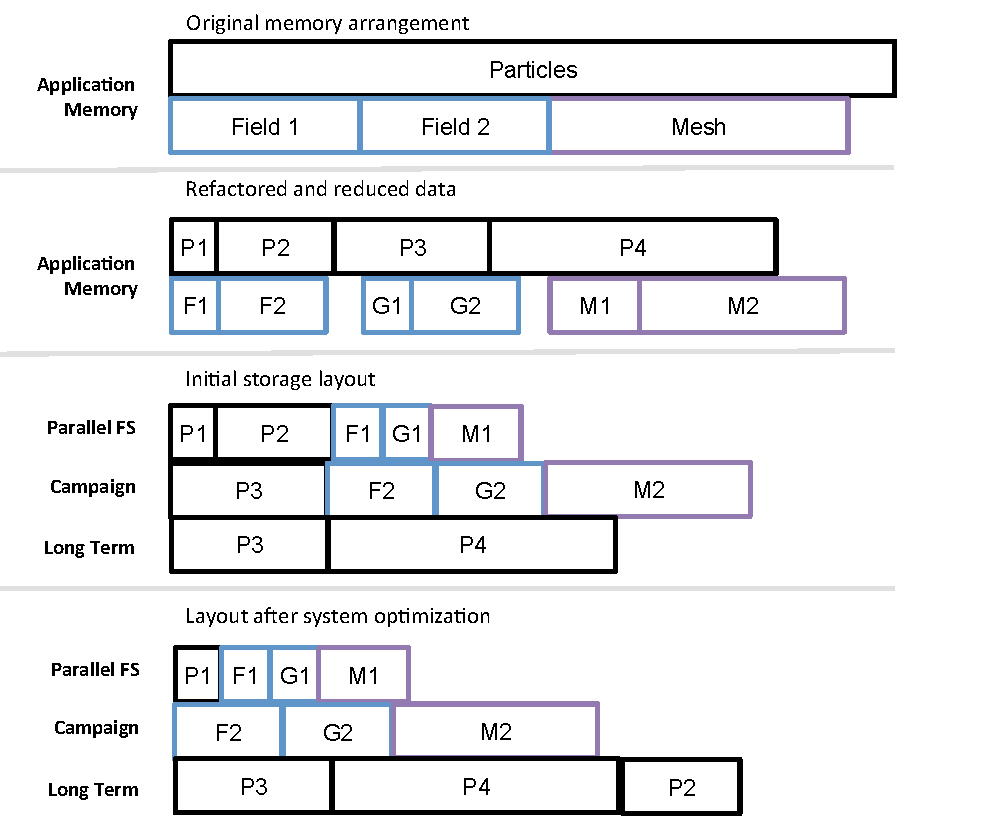
\includegraphics[scale=0.7]{graphics/SSIO-bucket.pdf}
        %\vspace{1ex}
        \caption{An illustration of SIRIUS managing data across the various stages of the data lifecycle.}
        \label{fig:ssio-bucket}
        \end{centering}
      \vspace{-1ex}
\end{wrapfigure}
%\lipsum[1]

We will explore the space of application level hints that can be easily provided
to SIRIUS. These hints will enable SIRIUS to make the
most appropriate optimization decisions for specific users in the context of the
multi-user environment rather than trying to rely on a one-size-fits-all
approach. In particular, we expect an application to provide hints on the
the time that an I/O operation will occur and
the expected data lifetime for output sets. For read calls we envision
hints that provide latency and precision requirements to the system. 

%In particular, the relationship to other chunks can
%be captured by including \textit{typed links}, each representing a different
%relationship type.  
In this project, a key set of metrics which will be stored as a metadata
attribute is \textit{data utility}.  It enables QoS scheduling, data placement
decisions, data lifetime decisions, and captures the value of the chunk to
the user. 
% It is
%our belief that exascale science will require users to prioritize a small set
%of chunks to be saved on higher-level capacity-limited storage to avoid the
%slow access to large-capacity lower-level storage, such as tape. 
% We propose a
%new technique, described by a \textit{utility function} provided by a user, where chunks
%can be cast into multiple data chunks and each bucket can be given a different utility value.  
Based on the utility, SIRIUS will construct the data description,
re-organize, and place the data to
achieve the desired QoS goals and policies.
 We will formulate the concept of utility (from an
application perspective) that is assigned to data chunks to quantify the
benefits of placement and/or movement actions to applications. These
utilities may be based on the importance of the data chunks, the frequency
with which they are accessed, etc., and can be used during runtime data
management to evaluate and compare different placement/movement options. 
For example, data chunks with higher utility value may be
placed closer (e.g., in faster memory) to the application.
Similarly, when it is time to evict data chunks from a higher storage
tier, the decision about which chunk to evict may take the utility into
account. Our initial work in defining such a utility is presented in~\cite{tongipdps15}.
 We will also explore autonomic approaches for balancing the placement and 
 movement of data across the memory hierarchy autonomically, which will be driven 
 by the data utility and will leverage both user hints and information gathered at runtime (e.g., runtime data access
history, network topology, etc.).

%
%A key insight in this proposed project will be the increased interaction of
%the application with the storage system.
%The users would like to have the ability to obtain information about, and even
%negotiate with the system to determine the
%level of QoS is possible given
%a prospective set of I/O operations and current state of the system, so that
%they can then make decisions about when and what data to access.

Towards this end, we propose to
address the QoS requirements by providing applications with mechanisms to
specify the quality of I/O service, interrogate the storage system, and react
to the responses. Guided by our past work we propose to explore the design of
the mechanisms for this purpose.  % In our example, the user will also request that
% the data in (P1, F1, G1, and M1) are given a higher bandwidth requirement than
% the other chunks of data. 
We will investigate how much additional information users
can provide at the time of writing in order for the system to place these chunks within
the QoS requirements. We will also investigate techniques which would allow the lowest
value chunks to never be written to the system if the time it takes to write exceeds the user
requirements.

We will also develop a querying mechanism that allows SIRIUS
to get estimated timing information of an I/O operation from the storage
system which can combine the information about data with system constraints
to provide a time estimate before the I/O operation is executed. 

% , which
% manages all storage resources and understands data via the data description, as well
% as system constraints such as the availability of storage space, before the I/O operation will
% be issued to the storage system. 
%This new query mechanism will allow users to
%adapt their applications to system dynamics, e.g., bandwidth/space fluctuations, and
%further reduce and expand data.

%We will explore how these query functions can be integrated into common applications with
%minimal code disruptions and a set of policies that applications can use to
%respond to these new information. For example, the user might  tell the system that
%the total time to write P, F1, F2, and the Mesh can never exceed 500 seconds. When the
%system sees that this can NOT be met, the system can drop P4 (for example), such that
%the time to write is met, and only the lowest value chunk is not written.

Users may also describe the data-refactoring routine by either requesting a system-provided
routine, or their application-aware plug-in which the user provides to the system. We will
create APIs for the plug-ins to use so that they will be unified in the way to create them
amongst all of the users. Plug-ins which are given back to the community may be 
eventually incorporated into a system-level plug-in if the community sees the benefit for
these more general plug-ins.

%Users will also need to describe information about the data in order to choose
%the optimal data-refactoring routine. Currently, we understand that
%users can tell us that the data represents: 1)~phase-space (e.g., the particles
%in our example), 2)~spatial-changes (e.g., the mesh), and 3)~space-time (e.g.,
%the fields on the mesh). We need this information to select
%the best possible data
%refactoring methods. Although users can insert a user-defined data-refactoring
%method, system-level methods can also use this information to make better decisions.
%We will investigate new techniques and new semantics capable of using
%this information to best prioritize and re-organize data.


% Removed the following because there are details on it.
%Finally, we will study the use of an external data annotation system that can
%provide information to the storage system without requiring recompilation of the application.


We will explore these techniques through the ADIOS
framework using many of our existing applications, including
XGC1~\cite{chang2006integrated}, GTC~\cite{klasky2003grid}, and SPECFM3D~\cite{SPECFEM3D}.
%We will design an API
%that will be integrated with the storage system to provide I/O time estimations so that
%users can decide which data priorities will be written and read. The utility
%value for each chunk will be used to sort the chunks into prioritized bins.
%Chunks in a particular bin will be assigned an appropriate storage
%tier and lifetime.
%As an example, Figure~\ref{fig:ssio-bucket} illustrates a use case for the XGC1 code.
%The user can pick a data-refactoring scheme (see
%\S~\ref{sec:data-refactor}) which will classify the particle data into four different
%value levels. The user can then pick a data utility, such as three months
%for the highest value level and twelve months for the lowest value level.
%The user will then specify all of the chunks one wants
%to write (particles, two fields, and a mesh in this example) and the system
%will return a time estimate for these write operations -
%in the case that this time estimate is too high, the user may
%compromise by specifying the highest value element to be written, skipping the rest in order to save time.
%Then the data will be placed
%onto the storage tiers, where for example the two highest value buckets
%will be stored in the Parallel File System, and the next highest value items
%will be placed to a lower tier within the storage hierarchy. 
%Depending on the capabilities of the actual storage system, 
%our proposed system will decide if the data will go through the parallel file system 
%towards a lower tier or can be staged to that tier directly. 
% Description of the utility function research

%An important research question that we must address is the semantics of
%describing the utility function, and the possibility that the users will
%accept this, and if the system can then use this information, and make 
%decisions based on this utility function. We realize that the system will
%try to optimize across all of the different user request, and the utility
%function must have defaults that users can see and change
%when the defaults would have a possible negative impact on
%their knowledge discovery. 

%The assumptions which we will make in choosing a utility function is that:
%1) There will only be a small number of priority levels that users will use
%to re-prioritize their data; 2) The number of tiers in the storage system will
%be small (e.g. NVRAM, PFS, Campaign Storage, HPSS), 3) The default
%lifetime of objects in each tier will be specified by the resource by
%a tuple (size, lifetime).  The user can then utilize this information to
%place information to the system such as: store the highest priority data
%as high up on the hierarchy for 6 months, and then migrate this data to tape.
%The user can also define the utility for CR files as that they have high
%priority but their lifetime is for a short period of time; i.e. when the
%next CR file appears on the system or the next two CR files. Research in
%describing this utility function will be in conjunction with users
%and we will evaluate how policies can be placed in the system and how well
%this utility function can be observed by the user.
 

Finally, we will explore a complementary notion of utility from a system-wide perspective 
that will capture and quantify, for example, the impact of placement decisions on 
the overall utilization of storage across multiple applications, and will enable system level runtime optimization. 
%\begin{wrapfigure}{R}{0.6\textwidth}
%        \begin{centering} 
%        \vspace{-4ex}
%	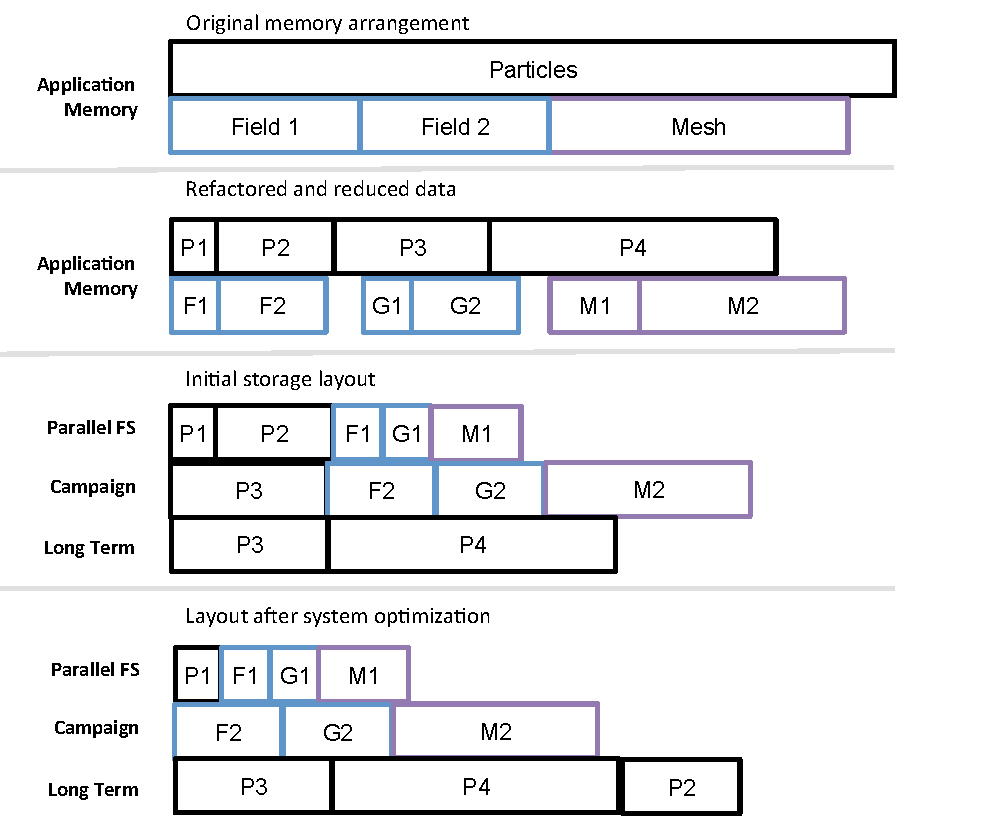
\includegraphics[scale=0.7]{graphics/SSIO-bucket.pdf}
%        %\vspace{1ex}
%        \caption{The system manages the data across the various stages of the data lifecycle}
%        \label{fig:ssio-bucket}
%        \end{centering}
%      \vspace{-1ex}
%\end{wrapfigure}
%\lipsum[1]


%
%
%
%We will design new techniques, available to both users and the storage system,
%to raise or lower these sub-chunks up and
%down the storage stack. The SSIO layer will then manage the system metadata so
%that the user can transparently access any of these sub-chunks without
%the need to know where the data currently resides.
%At read time, the middleware will be required to 
%provide a time estimate, and then allow the users to decide if
%they will read less (e.g., only the highest value sub-chunks)
%if the time estimate
%for reading does not meet requirements. Existing Sirocco functionality may be
%sufficient for these purposes, but it must still be proven in practice.
%

%
%
%Finally we will investigate the use of additional information
%on top of the data model.
%This information will be used to indicate data associations that exceed
%traditional data models. For example, the fields and mesh in our example have
%an inherent relationship. A common data model will describe all of the
%variables in the mesh (the coordinates, the units, and the types of elements if
%this were a finite-element mesh). We will explore new mechanisms that will
%group data together making it explicit that M1, F1, and G1 need to be organized
%together.  In other words, it will not be helpful if data from M1 and M2 were
%organized together along with only F1. When the users wants to visualize data
%from the field, F1, they will need only M1, and M2 would be additional
%information. Likewise, if the user wants to see F1 and F2, then they will need
%the mesh from M1 and M2. This requires that the time to access all of this
%data is approximately the same.
%We will investigate what choices the SSIO system must make in order to
%keep these pieces "together,'' from a performance perspective. Can the storage
%system move everything to a lower layer when all of it doesn't fit, or is there
%other, less tightly related data that can be evicted to preserve the collective
%retrieval performance?  We need to investigate the potential problems when this
%occurs and how the users can specify additional information to ensure they get
%the best possible data from the SSIO layer.

%We seek to provide dynamic runtime information to the user and make the
%system more transparent. This would allow the end user to analyze or
%visualize data in a more
%predictable way since they would have more confidence of how much time
%the data retrieval process would take.

%Firstly, we will explore the augmentation of I/O application programing
%interfaces (I/O APIs) to allow applications to both specify timing and quality
%information and also query the storage system for timing estimates. If user
%decide to write or read data to or from hierarchical storage systems, they
%will rely on the API to send their intentions for inquiry and examine the
%system status, including how much data they would like to write/read, desired
%bandwidth, data compression method, etc, or the user can express their
%intension of writing data right now no matter what the traffic is now.
%Through this interface we expect the application and user to gain insights
%into how long a single output or input call will take given the required
%quality information, and then react to these estimates by adjusting the
%quality or restricting the scope of the data required. Likewise we will
%explore how an application can provide timing information to the storage
%system to allow the storage system to make optimization decisions to best meet
%the requirements from the application. 
%
%Secondly, we will also explore external data annotations, such as those
%provided by the configuration file in ADIOS. Through the use of these external
%augmentation the user can provide insights to the storage system on the
%relative value of the data, expected life time and performance
%characteristics, as well as relationships between different data sets. With
%this information the storage system can make optimizations specific to a use
%case. We expect these augmentations to be particularly important for eviction
%of data from a storage layer, and migration of data sets to a different
%storage layer. 

\paragraph{Challenges:}
These new techniques offer both technical and adoption challenges. We will only
consider the technical challenges. The proposed techniques and features aim to
expose broad system level environmental information to the application and
allow the application to adapt dynamically based on this information.  One
aspect of this challenge is the design of an interrogative API that offers a
negotiation between the application and the storage system to make adaptation
decisions.  Since we will work closely with many of the leading LCF
applications, we need to make sure that our additional APIs and semantics in
the storage layer will be accepted by these applications and eventually by the
rest of the community. This requires careful examination of the full range
of possible
design choices to ensure stable APIs and useful semantics.



%%% Local Variables:
%%% mode: latex
%%% TeX-master: "../proposal"
%%% End:
